\documentclass[conference]{IEEEtran}
\IEEEoverridecommandlockouts

\usepackage{amsmath}
\usepackage{booktabs}
\usepackage{cite}
\usepackage{graphicx}
\usepackage{url}

\begin{document}

\title{Preliminary Evaluation of MeshEcho Confidence-Aware Routing for Airtime-Constrained LoRa Mesh IoT Networks}

\author{
\IEEEauthorblockN{Anonymous Authors}
\IEEEauthorblockA{Paper submitted to ICCT 2026 Track 8: Internet-of-Things \& Sensor Networks}
}

\maketitle

\begin{abstract}
LoRa mesh networking is attractive for low-power Internet-of-Things (IoT)
deployments that need wider coverage than a single hop can provide. However,
multi-hop LoRa routing has an inherent reliability-airtime tension: redundant
flooding improves reachability but increases channel occupancy, while cached
source routes reduce transmissions but can fail when a selected path contains a
weak or stale hop. This paper presents a preliminary packet-level evaluation of
that tradeoff for small LoRa mesh IoT networks. We build a reproducible
simulator with a LoRa time-on-air model, log-distance path loss, log-normal
shadowing, half-duplex radios, collision/capture behavior, and probabilistic
reception from SNR margin. Using this harness, we compare managed flooding, a
    source-route cache baseline, and a lightweight confidence-aware routing
    prototype, MeshEcho, that ranks discovered paths and uses bounded recovery
    forwarding for route-recovery cases. In the frozen 50-node mixed-traffic matrix, MeshEcho
    reaches 0.735 ACK-confirmed unicast PDR versus 0.389 for the source-route
    baseline, with 839.6 s versus 971.5 s of aggregate airtime. A paired cache-
    lifetime audit shows that matching the source-route baseline's cache TTL to
    MeshEcho's 600 s raises its ACK PDR to 0.519, reducing the native mean gap
    by 0.138 while leaving a 0.209 ACK-PDR gap in the matched bundle comparison.
    A separate
    controlled route-conflict experiment shows that the route-selection gain
    appears only when the shorter candidate contains a materially weaker hop:
    with 7.5 dB extra loss on that hop, MeshEcho reaches 0.999 ACK-confirmed
    PDR versus 0.784 for a shortest-path ablation, whereas null, moderate, and
    reverse controls produce no gain. The evaluation also exposes important
    fairness boundaries: fixed repeated pairs favor route caching, the default
    link setting is link-quality saturated and produces very few multi-hop
    routes, and adaptive recovery is not budget-matched across all protocol
    variants. A current-code recovery audit shows that disabling route-miss
    fallback changes ACK PDR by only $+0.009\pm0.018$ in a paired 20-seed
    replay, but does not make the baseline recovery budgets identical. These
    results support a bounded preliminary claim rather than universal
    dominance.

    An additional ten-seed, one-shot random-pair probe with timeout retries
    disabled for Smart-CALM gives MeshEcho 0.413 ACK-confirmed PDR and 97.5 s
    of airtime, versus 0.456 PDR and 139.5 s for source-route caching. Smart-CALM
    and its no-confidence control reach 0.489 and 0.488 PDR, respectively, with
    a paired 95\% interval for their difference that includes zero. Thus, the
    efficiency advantage persists outside the frozen matrix, but a general
    confidence-ranking advantage is not established.
\end{abstract}

\begin{IEEEkeywords}
LoRa mesh, Internet of Things, sensor networks, adaptive routing, airtime efficiency, packet delivery ratio
\end{IEEEkeywords}

\section{Introduction}

LoRa radios are widely used in low-power IoT systems because they provide long
communication range at modest device cost and energy consumption
\cite{augustin2016study}. Recent surveys and overview articles show that
multihop LoRa/LoRaWAN networking can relax star-topology constraints, but it
must manage airtime, link variability, and control overhead carefully
\cite{wong2024multihop,cotrim2020lorawanmesh,osorio2020routing,centelles2021beyond}.
In many deployments, terrain, indoor attenuation, transmit-power limits, and
gateway placement constraints can leave coverage gaps. LoRa mesh networking
addresses this by allowing intermediate devices to relay packets across
multiple hops for environmental sensing, temporary field monitoring, emergency
communication, and community-scale telemetry.

The challenge is that LoRa's low data rate and long packet time on air make
redundant forwarding expensive. A flooding-oriented design can reach many
nodes, but every rebroadcast consumes scarce airtime and raises collision
pressure. A source-route cache can reduce repeated transmissions, but a cached
route is only useful while its weakest hop remains good. This creates a
practical design question for LoRa mesh IoT networks:

\begin{quote}
How much forwarding redundancy should a node spend when path quality is
uncertain and airtime is scarce?
\end{quote}

Recent protocol studies explore several points in this design space, including
distance-vector LoRa mesh routing, reusable mesh libraries, spreading-factor
clustering, low-latency multihop forwarding, and real-time industrial LoRa
communication
\cite{pueyo2024minimalistic,sole2022implementation,zhu2019improving,ahmar2022smarthop,leonardi2023mrt}.
This paper studies the question as a preliminary routing-system evaluation. We
compare two fixed-mode baselines with a lightweight confidence-aware protocol
named MeshEcho. MeshEcho is the name of our protocol and is not a fork of
Meshtastic or MeshCore. The prototype is intentionally conservative: it does
not claim to solve all adaptive LoRa mesh routing problems. Instead, it
evaluates whether modest path confidence information can expose a better
operating point between managed flooding and pure source-route caching.

The contributions of this paper are:
\begin{itemize}
    \item We present a reproducible packet-level LoRa mesh simulation harness
    that evaluates routing policies under common topology, traffic, PHY,
    propagation, collision, and airtime assumptions.
    \item We characterize the reliability-airtime tradeoff between managed
    flooding and cached source routing in repeated-unicast and mixed IoT traffic.
    \item We evaluate MeshEcho, a preliminary confidence-aware routing
    protocol that ranks candidate routes using local link-quality evidence and
    limits fallback flooding to bounded recovery cases.
    \item We separate general random-topology results from a controlled
    route-conflict experiment with null and reverse controls, making the
    mechanism claim and its fairness boundary explicit.
\end{itemize}

The scope is deliberately preliminary. We focus on simulation-based evidence and
small-scale protocol characterization for ICCT Track 8. The implementation
reports the reproducible \texttt{calm-mesh} line as MeshEcho; the later online
Smart-CALM controller is treated as an exploratory extension rather than as the
main claim of this manuscript. A more complete firmware-oriented controller and
broader system validation are left for future work.

\section{Background and Motivation}

\subsection{LoRa Mesh Routing Tradeoffs}

LoRa modulation trades data rate for link budget. For IoT sensing, this is often
acceptable because payloads are small and traffic is intermittent. In a mesh,
however, each relay repeats the same low-rate packet. A route with several hops
therefore consumes multiple packet airtimes, and a flood can multiply this cost
across many relays.

Current LoRa mesh systems often operate near one of two routing extremes. A
managed-flooding approach rebroadcasts packets with randomized delays and
duplicate suppression. This is robust because delivery does not depend on one
chosen path, but it can generate many transmissions. A source-route cache first
discovers a path and then reuses it for later unicast packets. This reduces
redundant forwarding when traffic pairs repeat, but can be brittle if the first
discovered path includes a weak hop.

The same tension appears in low-power and lossy network routing more broadly.
RPL uses objective functions and routing metrics for constrained networks
\cite{rfc6550}, while ETX-style metrics showed that path selection should
consider delivery probability rather than hop count alone \cite{decouto2003etx}.
LoRa mesh differs in that airtime is particularly expensive and packets are
long enough for collision pressure to dominate at modest traffic levels. This
motivates a routing policy that treats redundancy as a limited resource rather
than as a fixed protocol behavior.

\subsection{Design Goal}

Our design goal is not to maximize reliability at all costs. Instead, we seek a
policy that can:
\begin{enumerate}
    \item keep the efficiency benefit of source routing when a path appears
    sufficiently reliable,
    \item avoid accepting obviously weak discovered paths when alternatives are
    available, and
    \item use bounded fallback forwarding only when route discovery or route
    confidence indicates uncertainty.
\end{enumerate}

This framing is suitable for IoT and sensor-network settings where traffic is
light enough for multi-hop LoRa to be useful, but dense enough that unnecessary
rebroadcasts still reduce network capacity.

\section{System Model}

\subsection{Network and Radio Model}

We simulate $N$ LoRa nodes uniformly placed in a square area. Nodes share one
half-duplex LoRa channel and may relay packets unless explicitly configured
otherwise. The default radio profile uses spreading factor SF9, bandwidth
125 kHz, coding-rate index 1 (4/5), 32-byte payloads, 17 dBm transmit power,
and a capture threshold of 6 dB, matching a representative SX126x-class LoRa
radio configuration \cite{semtech2024sx1262}.

Packet time on air follows the standard LoRa symbol-time calculation
\cite{semtech2013lora}. For spreading factor $SF$, bandwidth $BW$, payload
length $PL$, coding-rate index $CR$, explicit header flag $IH$, CRC flag $CRC$,
and low-data-rate optimization flag $DE$, the symbol time is
\begin{equation}
T_{sym}=\frac{2^{SF}}{BW}.
\end{equation}
The packet time on air is the preamble time plus the payload symbol time:
\begin{equation}
T_{oa}=(N_{pre}+4.25)T_{sym}+N_{payload}T_{sym},
\end{equation}
where $N_{payload}$ is computed using the standard LoRa payload-symbol
expression. The simulator accumulates total airtime by adding $T_{oa}$ for each
transmitted packet.

Propagation uses log-distance path loss with log-normal shadowing:
\begin{equation}
PL(d)=PL_0+10n\log_{10}(d/d_0)+X_\sigma,
\end{equation}
where $n$ is the path-loss exponent and $X_\sigma$ is a zero-mean Gaussian
shadowing term. The received power is $P_r=P_t-PL(d)$. The receiver noise floor
uses thermal noise plus a fixed noise figure. The simulator maps SNR margin to
packet reception probability through a logistic function:
\begin{equation}
P_{rx}=\frac{1}{1+\exp(-k\Delta_{SNR})},
\end{equation}
where $\Delta_{SNR}$ is the difference between measured SNR and the required
LoRa SNR threshold for the configured spreading factor. When transmissions
overlap, a receiver applies a capture rule: the desired packet can survive only
if it is at least the capture threshold stronger than the strongest interferer.
For tractability, all packet kinds use the same configured payload length in
the current simulator. Source-route header growth and protocol-specific
control-frame layouts are therefore not separately charged in the airtime
model.

\subsection{Traffic Model and Metrics}

We evaluate repeated unicast traffic, mixed traffic, and a separate random-pair
probe. Repeated unicast uses a fixed set of source-destination pairs so that
route caching has a meaningful opportunity to help. Mixed traffic contains both
unicast and broadcast flows, which is closer to many IoT mesh deployments that
combine telemetry, control, and local announcements. The random-pair probe
draws a new unicast source-destination pair for each application flow and is
used to test whether the frozen result depends on pair reuse.

The main metrics are unicast packet delivery ratio (PDR), broadcast coverage,
total transmissions, total airtime, airtime per delivery, and collision
failures. The frozen main matrix reports means over 20 random seeds, while the
random-pair probe reports means over 10 seeds as a fairness diagnostic. Each
seed changes node placement, traffic timing, selected pairs, the static
per-link shadowing realization, and stochastic reception outcomes. The frozen
main matrix also uses the historical shared random stream in which forwarding
jitter and reception draws can consume the same generator. The released
simulator provides an opt-in independent channel-randomness mode for new runs;
this separates reception draws from forwarding jitter and learning exploration,
but it still does not create event-by-event common random numbers when protocols
generate different numbers of transmissions. In the main matrix,
\texttt{unicast\_pdr} is the source-side ACK-confirmed delivery ratio;
destination DATA arrival is reported separately because destination reception
does not guarantee a successful ACK return. The main tables use the frozen
three-protocol matrix (managed flooding, source-route cache, and \texttt{calm-mesh});
the later Smart-CALM ablation files are retained as historical artifacts and
are not used for the quantitative claims in this paper. The comparison is a
common-harness comparison, not a claim that every protocol has identical
internal recovery semantics: MeshEcho has bounded fallback behavior, whereas
the two fixed baselines do not have an identical recovery controller.

\begin{figure*}[t]
\centering
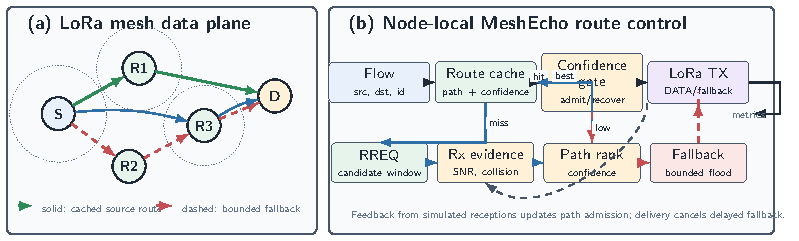
\includegraphics[width=0.98\textwidth]{figures/fig_calm_architecture.pdf}
\caption{Implemented MeshEcho routing architecture. Route discovery collects
candidate paths, receive evidence is converted to path confidence, and cached
source routes are supplemented only by bounded fallback forwarding when path
confidence or route availability is insufficient.}
\label{fig:architecture}
\end{figure*}

\section{Routing Policies}

\subsection{Managed Flooding Baseline}

The managed-flooding baseline models a Meshtastic-like forwarding behavior at a
protocol level \cite{meshtasticdocs}. A source transmits a data packet.
Relay-capable nodes that hear a new packet schedule a delayed rebroadcast. If a
relay hears another copy of the same packet before its scheduled transmission,
it suppresses its own forward. Packets stop when the destination receives them
or when the hop limit expires. This baseline represents a high-redundancy
operating point.

\subsection{Source-Route Cache Baseline}

The source-route baseline models a MeshCore-like path-cache behavior
\cite{meshcore}. If a source has no cached route to a destination, it floods a
route request (RREQ). The destination returns a route reply (RREP) along the
reverse discovered path. The source then caches the path and later unicast
packets carry the complete source route. Only the next hop on the source route
forwards the packet. This baseline represents a low-redundancy operating point.

\subsection{MeshEcho Confidence-Aware Prototype}

MeshEcho keeps the same basic route-discovery structure but changes how route
candidates are admitted.
During a short discovery window, the destination may observe multiple RREQ
paths. Instead of immediately accepting the first path, the prototype scores
candidate paths using simple local evidence from received packets. At a high
level, the score increases with stronger SNR margin and decreases with collision
evidence and additional hops. The selected route is cached with a finite
lifetime.

The prototype also includes bounded fallback forwarding. If no route is found,
the source sends a fallback flood to recover reachability. The implementation
also supports a confidence-triggered delayed fallback behind a source-routed
packet, which is canceled if the original delivery succeeds. In the frozen
\texttt{calm-mesh} matrix, the confidence threshold is set to zero, so the
reported CALM fallback counts are driven by route-recovery cases rather than by
an independently tuned confidence-triggered flood. Fallback is therefore a
small-radius recovery tool, not a permanent flooding mode.

This section intentionally describes only the preliminary MeshEcho mechanism
evaluated in this paper. More aggressive adaptive recovery and
implementation-specific control policies are outside the scope of this
submission.

\section{Experimental Evaluation}

\subsection{Setup}

Unless stated otherwise, simulations use 50 nodes in a $3000\,\mathrm{m} \times
3000\,\mathrm{m}$ square area, 1200 s duration, eight repeated unicast pairs,
maximum hop count 7, SF9, 125 kHz bandwidth, 32-byte packets, 17 dBm transmit
power, path-loss exponent 2.7, shadowing standard deviation 4 dB, and 20 random
seeds. Mixed traffic uses a mean offered load of six application packets per
minute. The high-shadowing stress case increases the shadowing standard
deviation to 6 dB. These settings define a reproducible common-harness
comparison, but they are not intended to represent every deployment density or
radio range. The repeated-pair workload is deliberately retained as a
route-cache efficiency case; it is not a neutral pair-churn workload. The
reported tables retain this frozen legacy matrix for traceability rather than
silently replacing it with a harder post-hoc parameter choice.

We performed a post-hoc calibration audit without replacing the frozen
results. Across 24,500 unordered node pairs, the minimum calculated direct-link
reception probability was 0.999909, with no pair below 0.99. The fixed-pair
minimum was 0.9999996 and remained 0.9999866 after an additional 8 dB
penalty. In the replayed main runs, 128 of 129 MeshCore cached routes and all
142 CALM cached routes were one hop. The matrix is therefore dominated by
contention and control traffic rather than multi-hop link-quality conflicts.
The static per-link shadowing realization is shared across protocols for each
seed, but temporal fading is not modeled. New fairness-oriented reruns should
enable the simulator's \texttt{--independent-rng-streams} option, while the
frozen files remain in legacy mode for exact reproduction of the published
numbers.

\subsection{Random-Pair Non-Saturated Multi-Hop Probe}

To test whether the preceding result depends on fixed-pair reuse and
link-quality saturation, we ran a separate ten-seed probe with 50 nodes in an
$18\,\mathrm{km} \times 18\,\mathrm{km}$ square. The probe uses random
source-destination pairs, mixed traffic at four application flows per minute,
SF7, 17 dBm transmit power, path-loss exponent 2.75, 4 dB shadowing, and the
independent channel-reception random stream. It is a fairness diagnostic rather
than a replacement for the frozen 20-seed matrix.

The mean per-seed direct-link PRR quantiles are 0.000026, 0.017577, 0.756816,
0.999517, and 1.000000 at the 5th, 25th, 50th, 75th, and 95th percentiles,
respectively. Fractions of direct links below 0.99 and 0.50 PRR are 0.642 and
0.443. The distribution is therefore non-degenerate, although some flows still
fail route discovery and the setting should not be treated as a calibrated
deployment model.

The Smart-CALM rows in Table~\ref{tab:randomprobe} use zero additional timeout
retries. This one-shot setting matches the timeout-retry budget across the
Smart-CALM variants, while retaining their declared routing and fallback
semantics. It is therefore a mechanism-control line, not a claim that all
protocols have identical native recovery controllers.

\begin{table*}[t]
\centering
\caption{One-shot, budget-matched random-pair, non-saturated multi-hop probe
over 10 seeds. Smart-CALM timeout retries are disabled. Values are means
$\pm$ half-widths of two-sided 95\% confidence intervals. The multi-hop-route
fraction is measured among completed cached routes; it is not defined for
managed flooding.}
\label{tab:randomprobe}
\scriptsize
\setlength{\tabcolsep}{3pt}
\resizebox{\textwidth}{!}{%
\begin{tabular}{lrrrrr}
\toprule
Protocol & ACK PDR & Destination PDR & Airtime (s) &
P95 ACK delay (s) & Multi-hop route fraction \\
\midrule
Managed flooding & 0.680$\pm$0.055 & 1.000$\pm$0.000 &
37.3$\pm$4.0 & 1.67$\pm$0.62 & -- \\
Source-route cache & 0.456$\pm$0.074 & 0.486$\pm$0.065 &
139.5$\pm$14.1 & 0.56$\pm$0.41 & 0.102 \\
MeshEcho & 0.413$\pm$0.117 & 0.479$\pm$0.108 &
97.5$\pm$10.2 & 2.49$\pm$0.08 & 0.434 \\
Smart-CALM & 0.489$\pm$0.122 & 0.557$\pm$0.132 &
98.7$\pm$10.3 & 3.07$\pm$0.43 & 0.449 \\
Smart-CALM-no-confidence & 0.488$\pm$0.090 & 0.566$\pm$0.096 &
97.5$\pm$10.3 & 2.97$\pm$0.38 & 0.328 \\
\bottomrule
\end{tabular}
}
\end{table*}

MeshEcho reduces airtime by approximately 30.1\% relative to source-route
caching in this probe, but its ACK PDR is 0.413 versus 0.456. Under the
one-shot budget, Smart-CALM reaches 0.489 ACK PDR and its no-confidence control
reaches 0.488. Paired by seed, the full-versus-no-confidence difference is
$+0.001$ with a 95\% confidence interval of $[-0.105,0.108]$; the
full-versus-no-fallback difference is $+0.024$ with
$[-0.041,0.090]$. Both intervals include zero. These results preserve the
airtime tradeoff but do not support an unconditional reliability or
confidence-ranking claim.

\begin{table*}[t]
\centering
\caption{Repeated-unicast results over 20 seeds. MeshEcho denotes the
confidence-aware prototype.}
\label{tab:unicast}
\begin{tabular}{lrrrr}
\toprule
Protocol & Unicast PDR & Total airtime (s) & Collision failures & Airtime reduction vs. flooding \\
\midrule
Managed flooding & 0.838 & 1152 & 120276 & -- \\
Source-route cache & 0.605 & 358 & 27488 & 68.9\% \\
MeshEcho & 0.831 & 256 & 17619 & 77.7\% \\
\bottomrule
\end{tabular}
\end{table*}

\begin{table*}[t]
\centering
\caption{Mixed-traffic and high-shadowing results over 20 seeds. MeshEcho
denotes the confidence-aware prototype.}
\label{tab:mixed}
\begin{tabular}{llrrrr}
\toprule
Scenario & Protocol & Unicast PDR & Broadcast coverage & Total airtime (s) & Collision failures \\
\midrule
Mixed traffic & Managed flooding & 0.852 & 0.947 & 1183 & 123501 \\
Mixed traffic & Source-route cache & 0.389 & 0.960 & 971 & 82454 \\
Mixed traffic & MeshEcho & 0.735 & 0.968 & 840 & 74103 \\
\midrule
High shadowing & Managed flooding & 0.842 & 0.952 & 1175 & 123322 \\
High shadowing & Source-route cache & 0.387 & 0.962 & 970 & 82324 \\
High shadowing & MeshEcho & 0.731 & 0.965 & 834 & 74129 \\
\bottomrule
\end{tabular}
\end{table*}

\begin{figure}[t]
\centering
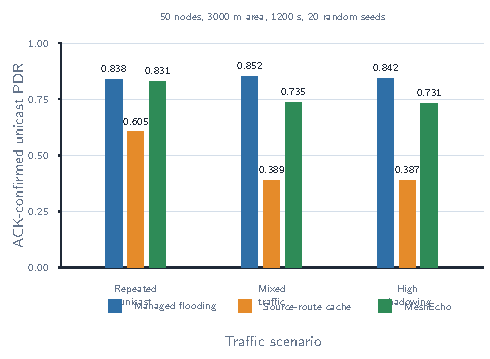
\includegraphics[width=\columnwidth]{figures/fig_unicast_pdr.pdf}
\caption{Unicast delivery ratio across the three evaluation scenarios.}
\label{fig:pdr}
\end{figure}

\begin{figure}[t]
\centering
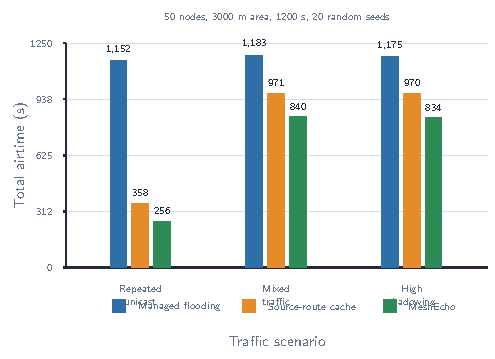
\includegraphics[width=\columnwidth]{figures/fig_total_airtime.pdf}
\caption{Aggregate LoRa airtime across the three evaluation scenarios.}
\label{fig:airtime}
\end{figure}

\subsection{Repeated Unicast}

Table~\ref{tab:unicast} and Figs.~\ref{fig:pdr}--\ref{fig:airtime} show the
repeated-unicast result. Managed flooding reaches the highest unicast PDR in
this scenario at 0.838, but spends 1152 s of aggregate airtime and produces
120,276 collision failures. Source-route caching reduces airtime to 358 s, but
its PDR drops to 0.605. MeshEcho reaches 0.831 PDR with 256 s of airtime and
17,619 collision failures. Thus, MeshEcho is close to flooding reliability in
    this particular repeated-pair setting while retaining most of the source-route
    efficiency. Because nearly all cached paths in this matrix are one hop, this
    result should not be interpreted as a general multi-hop route-selection
    result.

This scenario favors route caching because the same source-destination pairs
repeat. It is therefore a useful cache-efficiency case, but not a neutral
workload for protocols that do not rely on route reuse. The result should be
read as a tradeoff point rather than as evidence that MeshEcho dominates
flooding or generalizes to arbitrary pair churn. The separate random-pair probe
below reports pair churn together with a non-degenerate direct-link PRR
distribution and cached-route hop statistics.

\subsection{Mixed Traffic}

Mixed traffic is more challenging because broadcast and unicast flows share the
same channel. Table~\ref{tab:mixed} shows that the source-route baseline
maintains high broadcast coverage but has a lower ACK-confirmed unicast PDR of
0.389, compared with 0.852 for managed flooding. MeshEcho recovers part of
this loss, reaching 0.735 while reducing total airtime from 971 s to 840 s
relative to the source-route baseline. Collision failures decrease from
82,454 to 74,103.

    Compared with managed flooding, MeshEcho reduces airtime by 29.0\% and
    collision failures by 40.0\%, while keeping broadcast coverage within the same
    range. This end-to-end gain combines route admission and bounded recovery;
    it should not be attributed to confidence ranking alone. The remaining PDR
    gap to managed flooding indicates that the preliminary policy spends less
    redundancy but does not fully replace flood diversity.

\subsection{Recovery-Budget Sensitivity}

The frozen main matrix compares the CALM/MeshEcho bundle with a fixed
source-route baseline that has no equivalent route-miss recovery controller.
To quantify the contribution of this asymmetry, we reran the current code on
the same 20 seeds, topology-generation rule, traffic trace, and mixed-traffic
parameters while enabling the independent channel-reception stream. The only
change between the two CALM variants was whether a failed route discovery
could invoke route-miss fallback.

With fallback enabled, CALM reached 0.728 ACK PDR, 0.766 destination PDR, and
847.3 s of airtime. Disabling only route-miss fallback changed these values to
0.719, 0.744, and 831.4 s, respectively. The paired ACK-PDR difference was
$+0.009\pm0.018$ (two-sided 95\% t interval), while the paired destination-PDR
difference was $+0.023\pm0.023$. Fallback added 62.4 forwarding
transmissions and 15.9 s of airtime on average. Thus, route-miss recovery
contributes to the end-to-end result, but its mean ACK-PDR effect is small
relative to the full CALM-versus-MeshCore-like gap and is not statistically
separated from zero in this replay. The corresponding mean route-discovery
success rates were 0.798 with fallback, 0.805 without fallback, and 0.834 for
MeshCore-like. Thus, the headline CALM result is not explained by a higher
route-discovery success rate in this audit, although the native recovery
controllers are still not fully budget-matched. The audit is a sensitivity
check rather than a fully budget-matched baseline comparison.

\subsection{Route-Cache Lifetime Sensitivity}

The native configurations also use different route-cache lifetimes: 300 s for
MeshCore-like and 600 s for CALM/MeshEcho. Because the main workload reuses
eight fixed pairs, this difference can affect both route-discovery overhead and
the number of packets sent on an already discovered path. We therefore reran
the same 20 seeds with MeshCore-like at both 300 s and 600 s, while keeping
MeshEcho at 600 s.

The native 300 s MeshCore-like setting reached 0.381 ACK PDR, 0.652 destination
PDR, and 970.9 s of airtime. Matching its cache lifetime to 600 s increased
these values to 0.519, 0.722, and 905.5 s. The paired change was
$+0.138\pm0.031$ ACK PDR, $+0.070\pm0.034$ destination PDR, and
$-65.4\pm14.1$ s of airtime. Under the matched 600 s TTL, MeshEcho reached
0.728 ACK PDR and 847.3 s of airtime, giving a remaining paired difference of
$+0.209\pm0.071$ ACK PDR and $-58.2\pm19.2$ s of airtime. Thus, the native
headline comparison was materially favorable to MeshEcho because of the cache
TTL mismatch, although the matched audit still shows a protocol-bundle
difference. The frozen native matrix is retained for traceability; the matched
audit is the more appropriate fairness reference.

\begin{figure}[t]
\centering
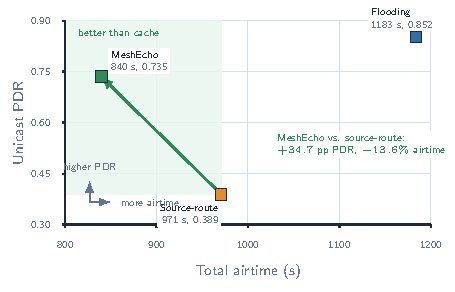
\includegraphics[width=\columnwidth]{figures/fig_tradeoff.pdf}
\caption{Mixed-traffic reliability-airtime tradeoff under the evaluated
protocol budgets. MeshEcho moves the source-route operating point toward higher
delivery with lower airtime, but the end-to-end difference includes bounded
recovery not available to the fixed baselines.}
\label{fig:tradeoff}
\end{figure}

\subsection{High-Shadowing Stress Case}

The high-shadowing case increases log-normal shadowing from 4 dB to 6 dB. The
same qualitative pattern remains, but the absolute values are not identical to
the mixed case. Source-route caching reaches 0.387 unicast PDR, while MeshEcho
reaches 0.731. Total airtime decreases from 970 s to 834 s and collision
    failures decrease from 82,324 to 74,129. This shows robustness of the
    aggregate configuration under stronger shadowing, but does not isolate
    confidence-aware admission because the random matrix still rarely creates a
    meaningful length-versus-quality conflict.

\subsection{Controlled Route-Conflict Ablation}

The random-topology matrix does not reliably create a direct conflict between
shortest-path and confidence ranking, so we use a separate controlled
experiment to test that mechanism. The topology has two candidate routes from
node 0 to node 5: a short path $0$--$1$--$2$--$5$ and a longer path
$0$--$3$--$4$--$6$--$5$. Non-edges are blocked explicitly. Each run uses
SF9, zero stochastic shadowing, a 12 s discovery window, a 1200 s route-cache
TTL, 24 unicast flows spaced by 30 s, and one route-discovery attempt. Online
learning, timeout retry, and route-miss fallback are disabled. The confidence
variant selects the highest-confidence candidate; the no-confidence variant
selects the shortest candidate.

The main mechanism condition adds 7.5 dB path loss to link $1$--$2$, while all
other permitted links receive no additional loss. The fairness audit also
contains a null condition, a moderate 5 dB short-branch condition, and a
reverse condition that weakens link $4$--$6$ on the long branch. Results are
paired by seed and use ACK-confirmed PDR.

\begin{table*}[t]
\centering
\caption{Controlled route-conflict fairness audit. Values are means over 100
paired seeds. The selected-route columns report the fraction of runs selecting
the indicated route class.}
\label{tab:conflict}
\scriptsize
\setlength{\tabcolsep}{3pt}
\resizebox{\textwidth}{!}{%
\begin{tabular}{lrrrrrr}
\toprule
Condition & MeshEcho PDR & No-confidence PDR & $\Delta$ PDR &
Long selected & Short selected & $\Delta$ airtime (s) \\
\midrule
No extra shadowing & 1.000 & 1.000 & 0.000 & 0.000 & 1.000 & 0.000 \\
Short branch +5 dB & 0.980 & 0.980 & 0.000 & 0.020 & 0.980 & 0.000 \\
Short branch +7.5 dB & 0.999 & 0.784 & +0.215 & 1.000 & 0.880 & +15.148 \\
Long branch +7.5 dB & 1.000 & 1.000 & 0.000 & 0.000 & 1.000 & 0.000 \\
\bottomrule
\end{tabular}
}
\end{table*}

Table~\ref{tab:conflict} shows that MeshEcho does not create a gain when the
two branches are effectively equivalent, and it does not blindly prefer the
longer route when the long branch is weakened. The 7.5 dB condition is
therefore evidence that the candidate-ranking mechanism can detect a
short-but-weaker path under this model. It is not evidence of
topology-independent superiority. The higher airtime in that condition also
shows the cost of selecting the reliable four-hop route instead of the
three-hop route. The moderate +5 dB condition is an important negative control:
the observed mean delta is zero, so the mechanism does not produce a gain for
every small perturbation.

\subsection{Route-Discovery Stress Check}

The connected-pair selector was also exercised separately to distinguish
multi-hop geometry from route-discovery operability. It selected a shared pool
of pairs at graph distance 2--4 using a static link-budget graph whose retained
edges had analytical PRR at least 0.90. In a 50-node, 15 km square with
24 pairs, SF7, and 0.5 flows per minute, MeshCore-like installed a route in
only 0.063 of route-discovery attempts and achieved 0.049 destination PDR.
A 20-seed single-flow check still gave a 0.050 discovery-success rate. The
RREP/RREQ transmission ratio was only 0.027 in the low-load run. We therefore
treat this configuration as a broadcast route-discovery stress test rather than
as evidence that source-route data forwarding is intrinsically inferior.
MeshCore-like also emits an RREP immediately upon first destination reception,
whereas MeshEcho waits for its candidate-collection window; in a
collision-limited flood, this reply-timing asymmetry can affect discovery
success. The corresponding raw rows and discovery diagnostics are released
separately from the headline comparison.

\section{Discussion}

The preliminary results support five observations. First, fixed flooding and
fixed source-route caching expose different sides of the LoRa mesh design
space. Flooding protects delivery but consumes substantial airtime. Cached
source routing saves airtime, but it can underperform when the selected route is
fragile. Because the default direct links are almost all high-PRR, the random
matrix should be interpreted primarily as a contention-oriented operating point,
not as a representative deployment-wide multi-hop calibration.

Second, route confidence is a plausible abstraction, but evidence for its
benefit comes primarily from the controlled route-conflict experiment. The
random-topology matrix does not estimate its average benefit reliably because
links are mostly high-PRR and cached paths are almost always one hop.

Third, the best operating point depends on traffic. In repeated unicast, route
caching is already strong and MeshEcho mainly improves efficiency. In mixed
traffic, its reliability gain over source-route caching includes bounded
    recovery unavailable to the fixed baselines. The current-code sensitivity
    audit estimates a small but nonzero mean effect from route-miss fallback
    ($+0.009\pm0.018$ ACK PDR), with a corresponding airtime cost. This remains
    a protocol-bundle result, not an isolated estimate of confidence ranking.
    Redundancy should therefore be treated as a per-context budget rather than
    a static network-wide mode.

Fourth, the random-pair probe changes the external-validity interpretation. In
the non-saturated multi-hop setting, MeshEcho retains lower airtime than the
source-route baseline but does not improve ACK PDR. After disabling additional
Smart-CALM timeout retries, the full and no-confidence variants are nearly
identical in mean ACK PDR, and their paired interval includes zero. Online
adaptation and confidence ranking should therefore not be presented as
general-purpose improvements from this probe. The probe is useful evidence
against overclaiming, not a replacement for a larger calibrated evaluation.

Fifth, the two experiments answer different questions: route-conflict isolates
admission under a known quality difference, while the random matrix measures
end-to-end behavior. The main matrix is a common-harness comparison, not a
fully budget-matched comparison of all recovery mechanisms; a mechanism study
must equalize route-cache lifetime, retry, and fallback budgets as well.

\section{Limitations and Future Work}

This work is a packet-level simulation rather than a physical deployment. The
model includes airtime, shadowing, probabilistic reception, half-duplex radios,
collision, and capture, but not full waveforms, duty-cycle regulation, real
firmware queues, or hardware sensitivity variation. The default 50-node,
3000 m, SF9 setting is a contention-oriented, high-PRR regime with almost no
multi-hop cached paths. Repeated unicast and the unicast component of mixed
traffic use eight fixed pairs. A separate ten-seed random-pair probe is included
to test this bias, but it has a harsh, partially disconnected operating point
and is diagnostic rather than a calibrated deployment study. Consequently,
the current data are not sufficient to claim calibrated multi-hop deployment
performance.

The comparison is fair at the common-harness level but not fully budget-matched:
MeshEcho has bounded fallback, while the fixed baselines have no identical
recovery controller. The new paired recovery audit shows that disabling
route-miss fallback changes the current CALM line by $+0.009\pm0.018$ ACK PDR
and $+0.023\pm0.023$ destination PDR, while reducing airtime by 15.9 s on
average. The one-shot random-pair probe disables additional
Smart-CALM timeout retries, so the confidence and no-confidence variants have
the same timeout-retry budget, but native fallback semantics remain different.
The native route-cache TTL is also 300 s for MeshCore-like versus 600 s for
MeshEcho; matching it to 600 s raises MeshCore-like ACK PDR by
$+0.138\pm0.031$ in the paired audit and reduces the remaining matched gap.
The separate two-retry Smart-CALM run is a recovery evaluation and is not used
as evidence for a confidence-only gain. Moreover, reception, forwarding
jitter, and exploration share one stream in the frozen matrix: same seeds fix
topology, traffic, and static shadowing, but not strict event-by-event common
random numbers. The released independent-stream option removes this particular
coupling for new reruns, but does not solve the different-transmission-count
problem. All packet kinds also use the same configured payload length, so
source-route header growth and control-frame format differences are omitted
from the airtime estimate. The connected-pair stress check also contains a
route-reply timing difference: MeshCore-like replies immediately, while
MeshEcho waits for candidate collection. This is another reason that the stress
check is not used as a neutral cross-protocol headline comparison.

The historical Smart-CALM ablation CSVs predate the no-fallback threshold fix
included in the released implementation and are not used for the main
quantitative claims. They remain in the repository only to preserve version
traceability; a fresh ablation rerun is required before interpreting those
variant rows.

The route-conflict ablation uses one seven-node topology, deterministic
permitted edges, zero stochastic shadowing, staggered route-request timing, and
a static channel. Its 100 seeds are repeated stochastic trials on that topology,
not 100 independent network layouts. The confidence estimate and subsequent
forwarding use the same static link realization, so stale or noisy confidence is
not tested. Finally, the comparison does not include a separately implemented
ETX or airtime-aware routing baseline.

Future work will expand the random-pair probe into a pre-registered full matrix,
calibrate a genuine multi-hop regime using direct-link PRR, route-discovery
success, and cached-route hop distributions, equalize retry and fallback
budgets, use the independent channel-random stream (or keyed per-event draws),
model variable packet headers, introduce time-varying links, and validate the
design with hardware-in-the-loop experiments.

\section{Conclusion}

This paper presented a preliminary evaluation of MeshEcho confidence-aware
routing for airtime-constrained LoRa mesh IoT networks. Using a reproducible
packet-level simulator, we compared managed flooding, source-route caching, and
the \texttt{calm-mesh} MeshEcho prototype. The results show that fixed routing
modes have clear operating boundaries: flooding is reliable but
airtime-intensive, while cached source routing is efficient but can lose
unicast reliability in mixed traffic. In the frozen 50-node mixed matrix,
MeshEcho reaches 0.735 ACK-confirmed unicast PDR with 840 s of airtime,
compared with 0.389 PDR and 971 s for source-route caching. The controlled
audit further shows that the route-ranking gain disappears under null,
moderate, and reverse controls, which bounds the mechanism claim to conditions
where link-quality evidence is informative. The one-shot random-pair probe
confirms the same boundary: MeshEcho keeps an airtime advantage but does not
show a PDR advantage over source-route caching, and Smart-CALM is nearly
identical to its no-confidence control. Because fixed pairs, limited probe
seeds, route-discovery stress cases, and unequal native recovery semantics
remain, these results should be read as preliminary common-harness evidence
rather than a universal ranking of LoRa mesh protocols.

\section*{Reproducibility and Declarations}
The MeshEcho simulator, routing implementation, experiment scripts, raw
results, and paper source are released in the accompanying repository:
\url{https://github.com/BH4ME/lora-mesh-routing-sim} (repository release
2.1.12). No human participants or personal data were involved. The authors
report no conflicts of interest and no external funding. Author contributions
cover protocol design, implementation, experiment design, analysis, and
manuscript preparation. AI-based tools assisted with code inspection and
language editing; the authors verified the implementation, numerical results,
and final manuscript.

\bibliographystyle{IEEEtran}
\bibliography{references}

\end{document}
